%!TEX root =  ./JanasJanssenCuffaro-August2019.tex

%SUBSECTION 2.5
\subsection{The singlet state, the Born rule and the elliptope} \label{1.5}

The correlation array in Figure \ref{CA-3set2out-Mermin} for our variation of the Mermin setup  can readily be produced in our quantum banana peeling and tasting experiment. In the end, the bananas, the peelings and the tastes are window-dressing for spin-$\frac12$ particles, measurements of their spin with Dubois magnets and outcomes of such measurements. Picking a pair of quantum bananas from our quantum-banana tree corresponds to preparing two spin-$\frac12$ particles in the singlet state, so called because its overall spin is zero. In the Dirac notation used from here on out we will designate this state as $|0, 0\rangle_{12}$ (see Eq.\ (\ref{singlet state s=1/2 simple}) below and Eq.\ (\ref{singlet state}) and note \ref{singlet note} in Section \ref{2.1}). The different peeling directions, $\vec{e}_a$, $\vec{e}_b$ and $\vec{e}_c$, correspond to different orientations of the axis of the Dubois magnets. The tastes, `yummy' and `nasty', corresponds to the spin values `up' and `down'. 

\begin{figure}[h!]
 \centering
   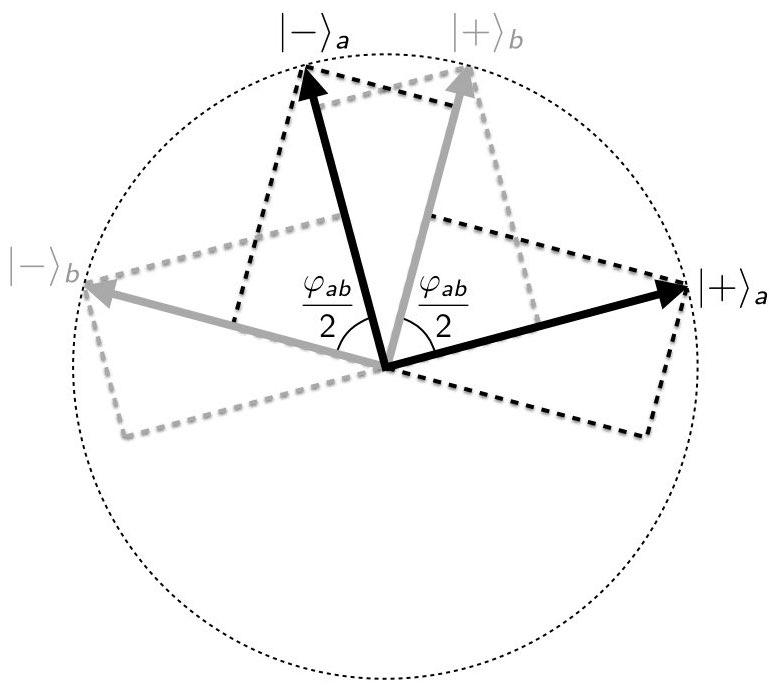
\includegraphics[width=3.5in]{vectors.jpeg} 
   \caption{Eigenvectors for the operators $\hat{S}_a$ and $\hat{S}_b$ acting on a one-banana Hilbert space and representing the tastes of the bananas when peeled being held in the directions $\vec{e}_a$ and $\vec{e}_b$, respectively.}
   \label{vectors}
\end{figure}

Sticking with the conceit of quantum bananas for now, we can say that the state $|0, 0\rangle_{12}$ is a vector in the Hilbert space for two bananas. This Hilbert space is the tensor product of two (identical) Hilbert spaces for one banana. The one-banana Hilbert space can be represented by the set of all vectors lying in the same plane and originating in the same point (see Figure \ref{vectors}). The properties `taste when peeled while being held in the direction of the unit vector $\vec{e}_a$' and `taste when peeled while being held in the direction of the unit vector $\vec{e}_b$' are represented by two operators, $\hat{S}_a$ and $\hat{S}_b$, acting in one-banana Hilbert space, respectively. Let $\{ | + \rangle_a, | - \rangle_a \}$ and  $\{ | + \rangle_b, | - \rangle_b \}$ be unit vectors that are eigenvectors of these operators with eigenvalues $\pm \bbar/2$:
\begin{equation}
\begin{array}{ccc}
\hat{S}_a \, | + \rangle_a = \displaystyle{\frac{\bbar}{2}} \, | + \rangle_a, & & \hat{S}_b \, | + \rangle_b = \displaystyle{\frac{\bbar}{2}}  \, | + \rangle_b,   \\[.4cm]
\hat{S}_a \, | - \rangle_a = - \displaystyle{\frac{\bbar}{2}}  \, | - \rangle_a, & \quad & \hat{S}_b \, | - \rangle_b = - \displaystyle{\frac{\bbar}{2}}  \, | - \rangle_b.   
\end{array}
\label{eigenvectors}
\end{equation}
Both sets of eigenvectors form an orthonormal basis for the one-banana Hilbert space. These eigenvectors are shown in Figure  \ref{vectors}. With malice aforethought, we have chosen the angle between  $|+\rangle_a$ and $|+\rangle_b$ to be half the angle $\varphi_{ab}$ between the unit vectors $\vec{e}_a$ and $\vec{e}_b$ in ordinary three-dimensional space.  

Using the orthonormal basis $\{ |+ \rangle_a, |- \rangle_a \}$ of one-banana Hilbert space, we can write the singlet state $| 0, 0 \rangle_{12}$  in two-banana Hilbert space as  
 \begin{equation}
| 0, 0 \rangle_{12} = \frac{1}{\sqrt{2}} \Big( |+ \rangle_{1a} |- \rangle_{2a} \, - \; |-  \rangle_{1a} | + \rangle_{2a} \Big)
\label{singlet state s=1/2 simple}
\end{equation}
(where the subscripts 1 and 2 refer to the bananas given to Alice and Bob, respectively). This is an \emph{entangled state}: the state vector for the composite system in the two-banana Hilbert space cannot be written as a tensor product of state vectors for its components in the two one-banana Hilbert spaces.

As we will see in Section \ref{2.1}, the singlet state, not just for a pair of spin-$\frac12$ particles but for a  pair of particles of arbitrary spin, is invariant under rotation. This means that $|0, 0 \rangle_{12}$ has the same form regardless of whether we use $\{ |+ \rangle_a, |- \rangle_a \}$ or $\{ |+ \rangle_b, |- \rangle_b \}$ as our orthonormal basis for the one-banana Hilbert space. Here we provide an intuitive proof of this property in the spin-$\frac12$ case. In Section \ref{2.1}, we prove this more rigorously for arbitrary spin.

Upon inspection of Figure \ref{vectors}, one sees that\footnote{What makes the proof in this section intuitive and dubious at the same time is that we take the coefficients in Eq.\ (\ref{QM2}) to be real whereas Hilbert space is a vector space over the complex rather than the real numbers. In Section \ref{2.1} (see Eqs.\ (\ref{Pauli matrices})--(\ref{b +/- trans law 2})), we will show that we can always write the eigenvectors of one spin operator as linear combinations \emph{with real coefficients} of the eigenvectors of another spin operator.}
\begin{equation}
\begin{array}{c}
|+ \rangle_a = \cos{\! \left( {\displaystyle \frac{\varphi_{ab}}{2}} \right)} \, |+ \rangle_b - \sin{\! \left( {\displaystyle \frac{\varphi_{ab}}{2}} \right)} \, |- \rangle_b, \\[.6cm]
|- \rangle_a = \sin{\! \left( {\displaystyle \frac{\varphi_{ab}}{2}} \right)} \, |+ \rangle_b + \cos{\! \left( {\displaystyle \frac{\varphi_{ab}}{2}} \right)} \, |- \rangle_b.
\end{array}
\label{QM2}
\end{equation}
Inserting these expressions into Eq.\ (\ref{singlet state s=1/2 simple}), we arrive at
\begin{align}
|0, 0 \rangle_{12} &= \frac{1}{\sqrt{2}} \Big\{ \! \left(  \cos{\! \left( \frac{\varphi_{ab}}{2} \right)}  |+ \rangle_{1b} - \sin{\! \left(  \frac{\varphi_{ab}}{2} \right)} |- \rangle_{1b} \! \right) \nonumber\\
& \qquad \quad \times \left(  \sin{\! \left(  \frac{\varphi_{ab}}{2}  \right)} |+ \rangle_{2b} + \cos{\! \left(  \frac{\varphi_{ab}}{2} \right)} |- \rangle_{2b} \!  \right) 
 \nonumber \\
  & \qquad \; - \left( \sin{\! \left(  \frac{\varphi_{ab}}{2}  \right)}  |+ \rangle_{1b} + \cos{\! \left(  \frac{\varphi_{ab}}{2}  \right)} |- \rangle_{1b} \right) \nonumber\\
 & \qquad \quad \times \!\! \left( \cos{\! \left(  \frac{\varphi_{ab}}{2}  \right)} |+ \rangle_{2b} - \sin{\! \left(  \frac{\varphi_{ab}}{2}  \right)} |- \rangle_{2b}  \right) \! \Big\}.  
 \nonumber
 \end{align}
Terms with $\sin{\!\left( \varphi_{ab}/{2} \right)} \cos{\!\left( \varphi_{ab}/{2} \right)}$ in this expression cancel; terms with $\cos^2{\!\left( \varphi_{ab}/{2} \right)}$ and $\sin^2{\!\left( \varphi_{ab}/{2} \right)}$ add up to:
\begin{equation}
|0, 0 \rangle_{12} = \frac{1}{\sqrt{2}} \Big( |+ \rangle_{1b} |- \rangle_{2b}  - |-  \rangle_{1b} | + \rangle_{2b} \Big), 
\label{QM3}
\end{equation}
 which has the exact same form as Eq.\ (\ref{singlet state s=1/2 simple}).   

To find the probabilities given by quantum mechanics for the four possible combinations of tastes found when Alice uses peeling direction $\vec{e}_a$  and Bob uses peeling direction $\vec{e}_b$, we need to write out $| 0, 0 \rangle_{12}$ in components with respect to the orthonormal basis:
\begin{equation}
\Big\{ |+ \rangle_{1a} |+ \rangle_{2b}, \; |+ \rangle_{1a} |- \rangle_{2b}, \; | - \rangle_{1a} | + \rangle_{2b}, \; |- \rangle_{1a} |- \rangle_{2b} \Big\}.
\label{QM4}
\end{equation}
These four basis vectors correspond to the four combinations of tastes Alice and Bob can find upon peeling their bananas. Using Eq.\ (\ref{QM2}) to express $|+ \rangle_{2a}$ and $|- \rangle_{2a}$ in Eq.\ (\ref{singlet state s=1/2 simple}) in terms of $|+ \rangle_{2b}$ and $|- \rangle_{2b}$, we find the singlet state in this new orthonormal basis:
\begin{eqnarray}
|0, 0 \rangle_{12}  & \! \! = \! \! & \frac{1}{\sqrt{2}} \Big( \sin{\! \left( \frac{\varphi_{ab}}{2} \right)} \, |+ \rangle_{1a}  |+ \rangle_{2b}  
\; + \;   \cos{\! \left( \frac{\varphi_{ab}}{2} \right)} \, |+ \rangle_{1a} |- \rangle_{2b} \nonumber \\
 &  & \quad \quad \quad \; - \;   \cos{\! \left( \frac{\varphi_{ab}}{2} \right)} \, | -  \rangle_{1a} | + \rangle_{2b}  
\; + \;   \sin{\! \left( \frac{\varphi_{ab}}{2} \right)} \, |-  \rangle_{1a} |- \rangle_{2b} \Big).
\label{expansion in ab}
\end{eqnarray}
We now use the \emph{Born rule}, the basic rule for probabilities in quantum mechanics, which in this case says that, when Alice peels $\hat{a}$ and Bob peels $\hat{b}$, the probabilities of them finding the combination of tastes `$++$', `$+-$', `$-+$' and `$--$', respectively, are the squares of the coefficients of the corresponding terms in the expansion of $| 0, 0 \rangle_{12}$ in Eq.\ (\ref{expansion in ab}).  It does not matter whose banana is peeled first (cf.\ note \ref{peeling order irrelevant}).

To find the probabilities for combinations of peeling directions other than $(\vec{e}_a, \vec{e}_b)$, we simply relabel $a$ and $b$ in Eq.\ (\ref{expansion in ab}) accordingly.  We thus see immediately that quantum mechanics correctly reproduces  the main features of the statistics of our banana-tasting experiment. If $ab$ is replaced by $aa$, $\varphi_{ab} = \varphi_{aa} = 0$ and Eq.\ (\ref{expansion in ab}) reduces to Eq.\ (\ref{singlet state s=1/2 simple}). If $ab$ is replaced by $bb$, Eq.\ (\ref{expansion in ab}) similarly reduces to Eq.\ (\ref{QM3}). Changing $a$ to $c$ in Eq.\ (\ref{singlet state s=1/2 simple}) or $b$ to $c$ in Eq.\ (\ref{QM3}), we likewise find the expansion of $|0, 0\rangle_{12}$ using the orthonormal basis $\{ | + \rangle_c,  | - \rangle_c \}$ of the one-banana Hilbert space. Applying the Born rule if the peeling combinations are $\hat{a}_A\hat{a}_B$, $\hat{b}_A\hat{b}_B$, or $\hat{c}_A\hat{c}_B$, we thus recover the perfect anti-correlation between the outcomes found by Alice and Bob whenever they peel their bananas the same way. Since $\varphi_{ab} = \varphi_{ba}$, $\varphi_{ac} = \varphi_{ca}$ and $\varphi_{bc} = \varphi_{cb}$, the Born rule also correctly predicts that having Alice and Bob swap peeling directions does not affect the probabilities of the various combinations of tastes. 

Thinking in terms of spin-$\frac12$ particles rather than bananas for a moment, we can now also present an intuitive argument as to why the angle between, say, $|+\rangle_a$ and $|+\rangle_b$ in Hilbert space is half the angle between the directions $\vec{e}_a$ and $\vec{e}_b$ in real space. Imagine we place two Dubois magnets in a beam of spin-$\frac12$ particles, one right after the other, with the second one rotated $180^{\mathrm o}$ with respect to the first. In this setup we would only find two possible outcomes $(+_1, -_2)$ and $(-_1, +_2)$ (where $\pm$ refers to spin up/down and 1 and 2 refer to the two Dubois magnets). The probability of finding $(+_1, +_2)$ and $(-_1, -_2)$, in other words, vanishes. For the Born rule to reproduce this result, the angle between the eigenvectors $|+\rangle_a$ and $|+\rangle_b$ should be $90^{\mathrm o}$ if the angle between the vectors $\vec{e}_a$ and $\vec{e}_b$ specifying two orientations of the Dubois magnet is $180^{\mathrm o}$. In Section 2.1, we will give a more general derivation of the relation between these two angles in the spin-$\frac12$ case (see Eqs.\ (\ref{rot proof 1})--(\ref{b +/- trans law 2})).

This argument, incidentally, reveals the limitations of the banana metaphor in two ways. First, we can only peel and taste a banana once. As Sandu \citet[p.\ vi]{Popescu 2016} put it in his foreword to \emph{Bananaworld}: ``once it's peeled it's peeled \ldots\ once it's eaten it's eaten.'' Secondly, there is an intrinsic difference between the tastes `yummy' and `nasty' of a banana (or, for that matter, between `heads' and `tails' of a quoin) whereas there is no intrinsic difference between `spin up' and `spin down'. `Spin up' and `spin down' are defined with respect some preferred axis, given, for instance, by the orientation of a Dubois magnet. 

This second complication also provides a simple argument for why we should not expect to succeed, using only elementary quantum systems as our components, in building a device such as the Superquantum Entangler PR01 of \citet{Bub and Bub 2018} realizing the PR box with the correlation array in Figure \ref{CA-PRbox}. Recall that the cells along the diagonal of the correlation array for this PR box are different. Now one can easily imagine that tossing two coins initially facing heads and tossing two coins initially facing tails would give different results. But this cannot be true for the spin-components of spin-$\frac12$ particles in the singlet state. Suppose we measure the spin-in-the-$z$-direction of both particles with two Dubois magnets. Spherical symmetry requires that the statistics for this experiment do not change if we rotate both Dubois magnets to measure, say, spin-in-the-$x$-direction. Measurements on the singlet state of two spin-$\frac12$ particles can thus not be used to produce a PR box with the correlation array in Figure \ref{CA-PRbox}. We will see below that they also cannot be used to produce a PR box for the Mermin setup with a correlation array represented by the point $\chi_{ab} = \chi_{ac} = \chi_{bc} = -1$ in Figure \ref{elliptope-LQPslice}.

\begin{figure}[ht]
 \centering
   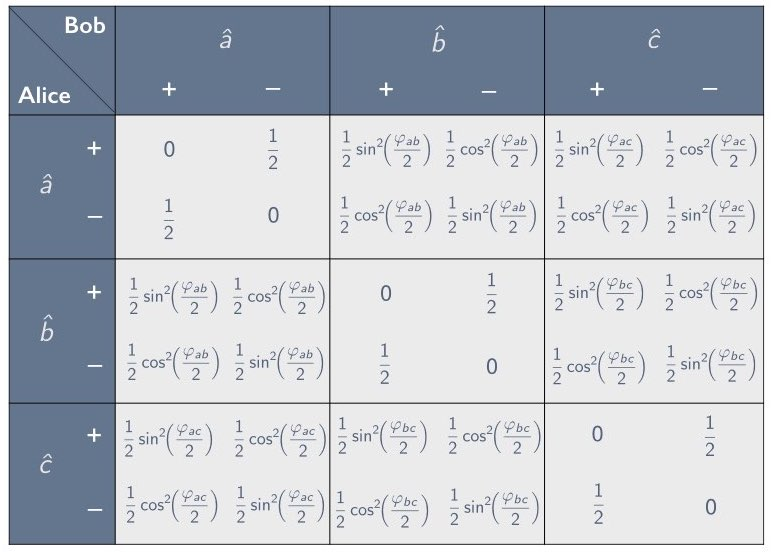
\includegraphics[width=4.5in]{CA-3set2out-non-signaling-halfangles.jpeg} 
   \caption{Correlation array given by quantum mechanics for two parties, one using settings $\hat{a}$ and one using setting $\hat{b}$, to perform a measurement on two spin-$\frac12$ particles in the singlet state.}
   \label{CA-3set2out-non-signaling-halfangles}
\end{figure}

With the help of Eq.\ (\ref{expansion in ab}) and the Born rule, we can fill out the correlation array for the Mermin setup. The result is shown in Figure \ref{CA-3set2out-non-signaling-halfangles}.  Note that the rows and columns of all cells add up to $\sfrac12$. The correlation array thus has uniform marginals. As we saw in Section \ref{1.2}, this is a sufficient condition for it to be non-signaling. 

In Mermin's setup (see Figure \ref{AliceBob-Mermin}), the peeling directions $\vec{e}_a$, $\vec{e}_b$ and  $\vec{e}_c$ corresponding to the settings $\hat{a}$, $\hat{b}$ and $\hat{c}$ are such that $\varphi_{ab} = \varphi_{ac} = \varphi_{bc} = 120\degree$. Inserting
\begin{equation}
\frac12 \sin^2{\! \left( \frac{\varphi_{ab}}{2}\right)} = \frac12 \sin^2{\! 60\degree} = \frac{3}{8}, 
\quad \frac12 \cos^2{\! \left( \frac{\varphi_{ab}}{2}\right)}  = \frac12 \cos^2{\! 60\degree} = \frac{1}{8}, 
\quad \mathrm{etc.,}
\end{equation}
in the correlation array in Figure \ref{CA-3set2out-non-signaling-halfangles}, we recover the Mermin correlation array in Figure \ref{CA-3set2out-Mermin}.

Using the trigonometric identities
\begin{equation}
\cos{\alpha} = \cos^2{\!\left( \frac{\alpha}{2} \right)} - \sin^2{\!\left( \frac{\alpha}{2} \right)} = 2 \cos^2{\!\left( \frac{\alpha}{2} \right)} -1 = 1 - 2 \sin^2{\!\left( \frac{\alpha}{2} \right)},
\label{trigonometry}
\end{equation}
we can replace the squares of sines and cosines of half the angles between peeling directions by cosines of the full angle. For instance,  
\begin{equation}
\frac12 \sin^2{\!\left(\frac{\varphi_{ab}}{2}\right)} = \frac{1}{4} \left( 1 - \cos{ \varphi_{ab}} \right), \quad
\frac12 \cos^2{\!\left(\frac{\varphi_{ab}}{2}\right)} = \frac{1}{4} \left( 1 + \cos{ \varphi_{ab}} \right).
\label{angle2halfangle}
\end{equation}
Comparison with the way we wrote the entries of a cell in a non-signaling array in Figure \ref{CA-2set2out-cell} then leads us to identify anti-correlation coefficients with these cosines:
\begin{equation}
\chi_{ab} = \cos{\varphi_{ab}}, \quad \chi_{ac} = \cos{\varphi_{ac}}, \quad \chi_{bc} = \cos{\varphi_{bc}}.
\label{chi values repeat}
\end{equation}

We can verify directly that $\chi_{ab} = \cos{\varphi_{ab}}$ by evaluating the expectation value $\langle \hat{S}_{1a} \, \hat{S}_{2b} \rangle_{00}$ of the product of the outcomes found by Alice and Bob when they use settings $\hat{a}$ and $\hat{b}$, respectively (cf.\ Eq.\ (\ref{prob 2 exp}); the subscript $00$ indicates that this expectation values is for systems in the singlet state $|0, 0 \rangle_{12}$). Recalling that the taste of a banana is $\pm \bbar/2$ and using the probabilities in the correlation array in Figure \ref{CA-3set2out-non-signaling-halfangles}, we find
\begin{eqnarray}
\langle \hat{S}_{1a} \, \hat{S}_{2b} \rangle_{00} & \!\! = \!\! & \frac{\bbar^2}{4} \left(\mathrm{Pr}(+\!+| \hat{a} \,\hat{b}) \, + \, \mathrm{Pr}(-\!-| \hat{a} \,\hat{b})\right) \nonumber\\
&&- \frac{\bbar^2}{4} \left(\mathrm{Pr}(+\!-| \hat{a} \,\hat{b}) \, + \, \mathrm{Pr}(-\!+| \hat{a} \,\hat{b})\right) \nonumber \\
&  \!\! = \!\! & \frac{\bbar^2}{4} \left(  \sin^2{\!\left(\frac{\varphi_{ab}}{2}\right)} - \cos^2{\!\left(\frac{\varphi_{ab}}{2}\right)} \right) \; = \; -\frac{\bbar^2}{4}\cos{\varphi_{ab}}.
\label{prob 2 exp b}
\end{eqnarray}
Using the standard deviations 
\begin{equation}
\sigma_{1a} = \sqrt{\langle \hat{S}^2_{1a} \rangle} = \bbar/2, \quad \sigma_{2b} = \sqrt{\langle \hat{S}^2_{2b} \rangle} = \bbar/2
\label{standard deviations a b}
\end{equation}
(cf.\ Eq.\ (\ref{standard deviations a and b})) and Eq.\ (\ref{chi as corr coef}) for $\chi_{ab}$, we find that 
\begin{equation}
\chi_{ab} \equiv  - \frac{\langle \hat{S}_{1a} \, \hat{S}_{2b} \rangle_{00}}{\sigma_{1a} \sigma_{2b}}  = \cos{\varphi_{ab}}. 
\label{chi2angle}
\end{equation}    

If the angles $\varphi_{ab}$, $\varphi_{ac}$ and $\varphi_{bc}$ could be chosen independently of one another the class of non-signaling correlation in our banana-tasting experiment allowed by quantum mechanics would saturate the non-signaling cube and we could realize the PR box represented by $\chi_{ab} = \chi_{ac} = \chi_{bc} = -1$. These angles, however, cannot be chosen independently of one another. 

To derive the constraint on the angles $\varphi_{ab}$, $\varphi_{ac}$ and $\varphi_{bc}$ , we introduce the \emph{matrix of anti-correlation coefficients} or \emph{anti-correlation matrix} $\chi$ for our version of the Mermin setup:
\begin{equation}
\chi
\equiv  
\begin{pmatrix}
\; 1 \; & \; \chi_{ab} \; & \;  \chi_{ac} \; \\[.2cm]
\; \chi_{ab} & \; 1 \; & \;  \chi_{bc} \; \\[.2cm]
 \; \chi_{ac} \; & \; \chi_{bc} \; & \;  1 
\end{pmatrix}
=
\begin{pmatrix}
\cos{\varphi_{aa}} & \cos{\varphi_{ab}} & \cos{\varphi_{ac}} \\[.2cm]
\cos{\varphi_{ab}} & \cos{\varphi_{bb}} & \cos{\varphi_{bc}} \\[.2cm]
\cos{\varphi_{ac}} & \cos{\varphi_{bc}} & \cos{\varphi_{cc}} 
\end{pmatrix}.
\label{chi matrix}
\end{equation}
Since the anti-correlation coefficients are given by these cosines, they can be written as inner products of the unit vectors in the associated peeling directions:
\begin{equation}
\chi_{ab} = \cos{\varphi_{ab}} = \vec{e}_a \cdot \vec{e}_b, \quad
\chi_{ac} = \cos{\varphi_{ac}} = \vec{e}_a \cdot \vec{e}_c, \quad
\chi_{bc} = \cos{\varphi_{bc}} = \vec{e}_b \cdot \vec{e}_c. \quad
\label{chis2angles2innerproducts}
\end{equation}
Such a matrix of inner products is called a \emph{Gram matrix}. Writing the components of the three unit vectors as
\begin{equation}
\vec{e}_a = (a_x, a_y, a_z),  \quad \vec{e}_b = (b_x, b_y, b_z), \quad \vec{e}_c = (c_x, c_y, c_z),
\label{comps of unit vectors e_abc}
\end{equation}
we can write this Gram matrix as
\begin{equation}
\chi
= 
\begin{pmatrix}
\vec{e}_a \! \cdot  \vec{e}_a &  \vec{e}_a \! \cdot  \vec{e}_b  &   \vec{e}_a \! \cdot  \vec{e}_c  \\[.2cm]
\vec{e}_b \! \cdot  \vec{e}_a & \vec{e}_b \! \cdot  \vec{e}_b & \vec{e}_b \! \cdot  \vec{e}_c \\[.2cm]
\vec{e}_c \! \cdot  \vec{e}_a & \vec{e}_c \! \cdot  \vec{e}_b  & \vec{e}_c \! \cdot  \vec{e}_c 
\end{pmatrix}
=
\begin{pmatrix}
\; a_x \; & \; a_y \; & \;  a_z \; \\[.2cm]
\; b_x \; & \; b_y \; & \;  b_z \; \\[.2cm]
 \; c_x \; & \; c_y \; & \;  c_z 
\end{pmatrix}
\begin{pmatrix}
\; a_x \; & \; b_x \; & \;  c_x \; \\[.2cm]
\; a_y \; & \; b_y \; & \;  c_y \; \\[.2cm] 
 \; a_z \; & \; b_z \; & \;  c_x 
\end{pmatrix}.
\label{QM10}
\end{equation}
Introducing
\begin{equation}
L \equiv
\begin{pmatrix}
\; a_x \; & \; b_x \; & \;  c_x \; \\[.2cm]
\; a_y \; & \; b_y \; & \;  c_y \; \\[.2cm]
 \; a_z \; & \; b_z \; & \;  c_x 
\end{pmatrix},
\label{QM11}
\end{equation}
we can write Eq.\ (\ref{QM10}) more compactly as
\begin{equation}
\chi = L^\top L.
\label{QM12}
\end{equation}
It follows that the determinant of $\chi$ is non-negative: 
%\citep[p.\ 515]{Deza and Laurent 1997}:
\begin{equation}
\det{\chi} = \det{\!(L^\top L)} = (\det{L^\top})(\det{L}) = (\det{L})^2 \ge 0. 
\label{QM13}
\end{equation}
Using Eq.\ (\ref{chi matrix}) to evaluate the determinant of $\det{\chi}$, we can rewrite this condition as
\begin{equation}
1 - \chi_{ab}^2 - \chi_{ac}^2 - \chi_{bc}^2 + 2 \, \chi_{ab} \, \chi_{ac} \, \chi_{bc} \ge 0.
\label{QM14}
\end{equation}

\begin{figure}[ht]
 \centering
   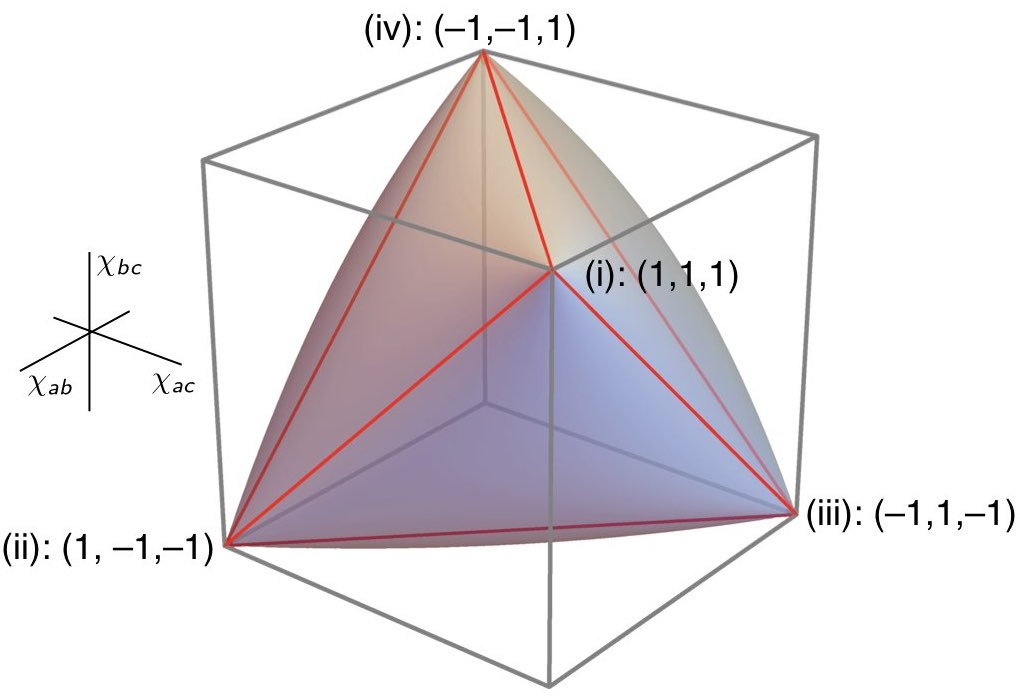
\includegraphics[width=4.5in]{elliptope.jpeg} 
   \caption{Elliptope of triplets of anti-correlation coefficients $(\chi_{ab}, \chi_{ac}, \chi_{bc})$ allowed by quantum mechanics in our version of the Mermin setup.}
   \label{elliptope}
\end{figure}

Eq.\ (\ref{QM14}) is the constraint we were looking for. Quantum mechanics only allows those non-signaling correlation arrays in Figure \ref{CA-3set2out-non-signaling-halfangles}  for which the anti-correlation coefficients that can be used to parametrize them (see Eqs.\ (\ref{angle2halfangle})--(\ref{chi values repeat})) satisfy this constraint. The region of the non-signaling cube picked out by Eq.\ (\ref{QM14})  is the elliptope in Figure \ref{elliptope}, an ``inflated'' version of the tetrahedron of classically allowed triplets of correlation coefficients in Figure \ref{tetrahedron}.\footnote{In Section \ref{1.3} we already showed the cross-section $\chi_{bc} = 0$ of the non-signaling cube, the elliptope and the classical tetrahedron (see Figure \ref{elliptope-LQPslice}).} 

It is easy to verify that the elliptope contains the classical tetrahedron. The vertices (i) through (iv) with the values
\begin{equation}
(1, 1, 1), \quad (1, -1, -1), \quad (-1, 1, -1), \quad (-1, -1, 1),
\label{vertices a}
\end{equation}
for $(\chi_{ab}, \chi_{ac}, \chi_{bc})$ all satisfy Eq.\ (\ref{QM14}) with an equality sign:
\begin{equation}
1 - \chi_{ab}^2 - \chi_{ac}^2 - \chi_{bc}^2 + 2 \, \chi_{ab} \, \chi_{ac} \, \chi_{bc} = 0.
\label{QM14a}
\end{equation}
So do the six lines connecting these four vertices. Consider the top and bottom face of the non-signaling cube, where $\chi_{bc} =1$ and $\chi_{bc} = -1$, respectively. Eq.\ (\ref{QM14a}) then reduces to:
\begin{equation}
- \chi_{ab}^2 - \chi_{ac}^2 \pm 2\, \chi_{ab} \, \chi_{ac} = 0.
\label{QM14b}
\end{equation}
So the line $\chi_{ab} = \chi_{ac}$ on the $\chi_{bc} =1$ face of the cube and the line $\chi_{ab} = -\chi_{ac}$ on the $\chi_{bc} =-1$ face of the cube satisfy Eq.\ (\ref{QM14a}). These are the lines connecting the vertices on these two faces of the cube. We similarly find that the other four lines connecting vertices of the tetrahedron satisfy Eq.\ (\ref{QM14a}): the $\chi_{ac} = \chi_{bc}$ line on the $\chi_{ab}=1$ face, the $\chi_{ac}=-\chi_{bc}$ line on the $\chi_{ab}=-1$ face, the $\chi_{ab}= \chi_{bc}$ line on the $\chi_{ac}=1$ face and the $\chi_{ab}=-\chi_{bc}$ line on the $\chi_{ac}=-1$ face.
 
The volumes of the tetrahedron and the elliptope are $\sfrac83$ and $\pi^2/2$, respectively, which means that their ratio is $.54$. By this metric, the class of correlations allowed quantum-mechanically in this setup is thus almost twice as large as the class of correlations allowed by local hidden-variable theories.     

Once again consider Eq.\ (\ref{QM14}). The constraint it expresses has a simple geometrical interpretation. Note that $\det{L} = \pm V$, where $V$ is the volume of the parallelepiped spanned by the three unit vectors $\vec{e}_a$, $\vec{e}_b$ and $\vec{e}_c$. If this triplet is positively oriented, $\det{L} = V$; if it is negatively oriented, $\det{L} = -V$. Consider the case that $\det{\chi} = (\det{L})^2 = 0$, which means that $V=0$. This, in turn, means that $\vec{e}_a$, $\vec{e}_b$ and $\vec{e}_c$ are coplanar. Hence, the statement that $\det{\chi} =0$ is equivalent to the statement that either the three angles $(\varphi_{ab}, \varphi_{ac}, \varphi_{bc})$ add up to $360\degree$ or one of them is the sum of the other two \citep[p.\ 515]{Deza and Laurent 1997}.

To verify this equivalence we use the trigonometric identity
\begin{eqnarray}
(2 \cos{\alpha}) (2 \cos{\beta}) (2 \cos{\gamma}) & \! \!  = \! \!  & 2 \cos{(\alpha + \beta + \gamma)}
+ 2 \cos{(- \alpha + \beta + \gamma)} \nonumber \\
 & & \quad  + \; 2 \cos{(\alpha - \beta + \gamma)} + 2 \cos{(\alpha + \beta - \gamma)}, 
\label{QM15}
\end{eqnarray}
which can easily be checked with the help of the Euler formula, $2 \cos{\alpha} = e^{i \alpha} + e^{-i \alpha}$. In all cases in which one of the angles $(\alpha, \beta, \gamma)$ is either the sum of the other two ($\alpha = \beta + \gamma$, $\beta = \alpha + \gamma$, or $\gamma = \alpha + \beta$) or is $360\degree$ minus this sum ($\alpha+\beta+\gamma=360\degree$), the right-hand side of Eq.\ (\ref{QM15}) reduces to
\begin{equation}
2 + 2 \cos{2 \alpha} + 2 \cos{2 \beta} + 2 \cos{2 \gamma}
= 4 \cos^2{\! \alpha} + 4 \cos^2{\!\beta} + 4 \cos^2{\!\gamma} - 4.
 \label{QM16}
\end{equation}
Eq.\ (\ref{QM15}) can thus be rewritten as
\begin{equation}
2 \cos{\alpha} \cos{\beta} \cos{\gamma} = \cos^2{\!\alpha} + \cos^2{\!\beta} + \cos^2{\!\gamma} - 1.
\label{QM17}
\end{equation}
Substituting $(\varphi_{ab}, \varphi_{ac}, \varphi_{bc})$ for  $(\alpha, \beta, \gamma)$ and $(\chi_{ab}, \chi_{ac}, \chi_{bc})$ for  $(\cos{\varphi_{ab}}, \break \cos{\varphi_{ac}}, \cos{\varphi_{bc}})$, 
%(see Eq.\ (\ref{chis2angles2innerproducts})), 
we see that Eq.\ (\ref{QM17}) reduces to Eq.\ (\ref{QM14}) with an `$=$' sign rather than a `$\ge$' sign. This shows that the equality $\det{\chi} =0$ is indeed equivalent to the statement that the angles $(\varphi_{ab}, \varphi_{ac}, \varphi_{bc})$ either add up to $360\degree$ or that one of them is the sum of the other two. More generally, the \emph{inequality} $\det \chi\geq 0$ is equivalent to the statement that either their sum is no larger than $360\degree$ or the sum of any two of them is no smaller than the third, i.e.,  
\begin{equation}
\begin{array}{c}
 \varphi_{ab} +  \varphi_{ac} + \varphi_{bc} \le 360\degree  \\[.2cm]
\mathrm{or} \;\; \big( \; \varphi_{ab} \le  \varphi_{ac} + \varphi_{bc} \;\; \mathrm{and} \;\; \varphi_{ac} \le  \varphi_{ab} + \varphi_{bc}  \;\;  \mathrm{and} \;\; \varphi_{bc} \le  \varphi_{ab} + \varphi_{ac} \; \big) 
\end{array}
\label{angle inequalities}
\end{equation}
\citep[p.\ 515; cf.\ the triangle on the right in Figure \ref{vectors4elliptope} in Section \ref{1.6}]{Deza and Laurent 1997}.
%\citep[for proof, see][p.\ 515]{Deza and Laurent 1997}. 
These angle inequalities can be represented geometrically by the tetrahedron in Figure \ref{tetrahedron-angles}.\footnote{These inequalities can also be found in \citet[remark on p.\ 170]{Accardi and Fedullo 1982}. These authors also give Eq.\  (\ref{QM14}) for the elliptope in terms of \emph{the cosines of} these angles, which are just our anti-correlation coefficients $(\chi_{ab}, \chi_{ac}, \chi_{bc})$ (ibid., p.\ 166, Eq.\ 19; p.\ 168, Eq.\ 33; p.\ 169, Eq.\ 37):
$$
2 \, \cos{\varphi_{ab}} \, \cos{\varphi_{ac}} \, \cos{\varphi_{bc}} \ge  \cos^2{\!\varphi_{ab}} + \cos^2{\!\varphi_{ac}} + \cos^2{\!\varphi_{bc}} - 1.
%\label{QM17a}
$$
Citing \citet{Accardi and Fedullo 1982}, Bas \citet[pp.\ 120--121]{Van Fraassen 1991} states this same inequality in terms of probabilities rather than correlation coefficients, just as Mermin did with the Bell inequality (see Section \ref{1.4}, Eqs.\ (\ref{Pr opp Mermin})--(\ref{Pr opp general})).\label{Accardi Fedullo}}  

\begin{figure}[ht]
 \centering
   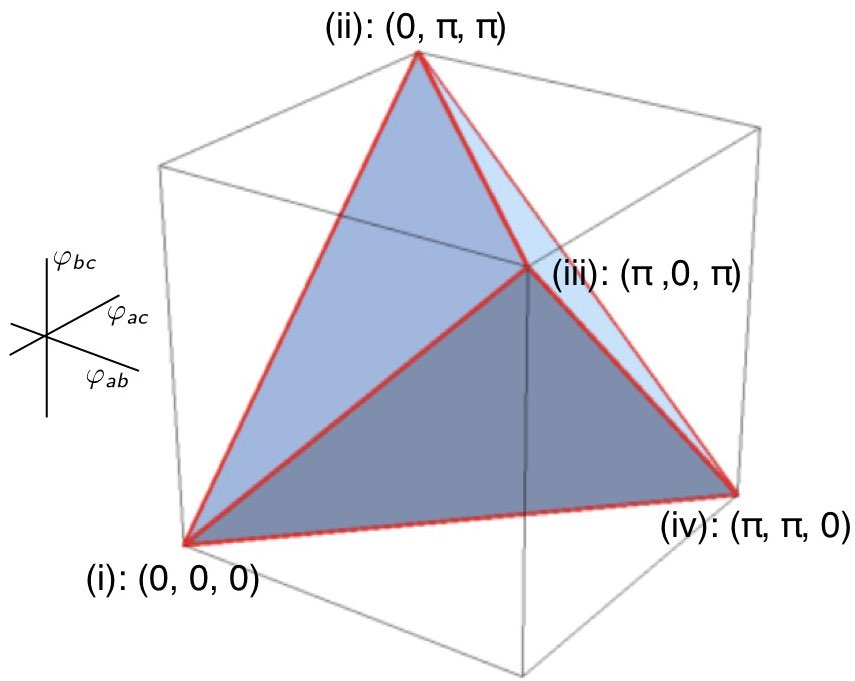
\includegraphics[width=4.5in]{tetrahedron-angles.jpeg} 
   \caption{Tetrahedron of triplets of angles $(\varphi_{ab}, \varphi_{ac}, \varphi_{bc})$ allowed by quantum mechanics in our version of the Mermin setup.}
   \label{tetrahedron-angles}
\end{figure} 

In the special case that Mermin considered, as we saw in Section \ref{1.3} (see Eq.\ (\ref{chi values Mermin example})),  
\begin{equation}
\chi_{ab} = \chi_{ac} = \chi_{bc} = -\sfrac12.
\label{chi values Mermin example repeat}
\end{equation}
In terms of the corresponding angles, this is the point
\begin{equation}
\varphi_{ab} = \varphi_{ac} = \varphi_{bc} = 120\degree
\end{equation}
at the center of the facet (ii)-(iii)-(iv) of the tetrahedron in Figure \ref{tetrahedron-angles}. 

At this point, the sum of the anti-correlation coefficients has its minimum value of $-\sfrac32$. This sum thus satisfies the inequality,
\begin{equation}
\chi_{ab} + \chi_{ac} + \chi_{bc} \ge -\sfrac32.
\label{Mermin Tsirelson bound on chis}
\end{equation}
This is the quantum analogue of the CHSH-type Bell inequality for local hidden-variable theories, which says that this quantity cannot be smaller than $-1$ (see Eq.\ (\ref{Mermin inequality CHSH-like})). The inequality in Eq.\ (\ref{Mermin Tsirelson bound on chis}) gives the \emph{Tsirelson bound} for this setup, named for Boris \citet{Cirel'son 1980}. Both the Tsirelson bound and the CHSH-type Bell inequality for this setup are represented by dotted lines in the cross-section of the quantum elliptope and the classical tetrahedron in Figure \ref{elliptope-LQPslice}.\footnote{The line marked ``Tsirelson bound'' in Figure \ref{elliptope-LQPslice} does not touch the circle representing the quantum convex set because the point $(\chi_{ab}, \chi_{ac}, \chi_{bc}) = (-\sfrac12, -\sfrac12, -\sfrac12)$ for which $\chi_{ab} + \chi_{ac} + \chi_{bc}$ reaches the minimum value quantum mechanics allows, lies below the plane $\chi_{bc}=0$ (cf. Figure \ref{elliptope}).} 

The point where the sum of the anti-correlation coefficients reaches the minimum value allowed by quantum mechanics in the Mermin setup is also the point where the probability of Alice and Bob finding opposite results reaches the minimum value allowed. Substituting the values for the anti-correlation coefficients in Eq.\ (\ref{chi values Mermin example repeat}) into Eq.\ (\ref{Pr opp Mermin}), we find
\begin{equation}
\mathrm{Pr(opp)} = \sfrac{2}{3} \, + \, \sfrac{1}{9} \, \Big(\chi_{ab} + \chi_{ac} + \chi_{bc} \Big) = \sfrac23 \, - \, \sfrac16 = \sfrac12.
\label{Pr opp Mermin (double)}
\end{equation}

As in the classical case (see Eqs.\ (\ref{Mermin inequality CHSH-like (i)})--(\ref{Mermin inequality CHSH-like (iv)})), we can write down three pairs of inequalities like the one for which the lower bound is given in Eq.\ (\ref{Mermin Tsirelson bound on chis}):  
\begin{equation}
-\sfrac32 \le \;\, \chi_{ab} - \chi_{ac} - \chi_{bc} \; \le 3, 
\label{Mermin Tsirelson bound on chis (ii)}
\end{equation}
\begin{equation}
-\sfrac32 \le - \chi_{ab} + \chi_{ac} - \chi_{bc} \le 3, 
\label{Mermin Tsirelson bound on chis (iii)}
\end{equation}
\begin{equation}
-\sfrac32 \le - \chi_{ab} - \chi_{ac} + \chi_{bc} \le 3.
\label{Mermin Tsirelson bound on chis (iv)}
\end{equation}
However, while the classical counterparts of these four linear inequalities sufficed to fully characterize the classical tetrahedron, we needed the non-linear inequality in Eq.\ (\ref{QM14}) to characterize the elliptope with its curved surface. 
